\newpage 
\chapter{ ساختار زمین ناقص و فراماده و تاثیر آنها بر کاهش تزویج}
\label{ch:3}
\section{مقدمه}
در این فصل با پیاده سازی ساختار ارائه شده در مقاله
\cite{carver1981microstrip}
و یک طرح فراماده مشهور تلاش بر کاهش کوپلینگ شده که در ادامه با توضیح هر کدام ساختار را برسی میکنیم.

\section{ساختار زمین ناقص}
ساختار زمین ناقص  با ایجاد نقص‌های مهندسی‌شده در صفحه زمین، توزیع جریان‌های سطحی را تغییر داده و باعث ایجاد خواص ممنوعه باندی
\LTRfootnote{Band-Stop}
 در پاسخ فرکانسی می‌شود. این ویژگی به‌طور مستقیم بر کاهش تزویج متقابل از طریق مهار انتشار امواج سطحی تأثیر می‌گذارد.
 
 
 ساختار DGS را می‌توان با یک مدار LC موازی مدلسازی کرد که در فرکانس رزونانس، امپدانس بالایی را ایجاد می‌کند و باعث مسدودسازی سیگنال می‌شود. مقادیر سلف ($L$) و خازن ($C$) به هندسه و ابعاد نقص ایجاد شده در صفحه زمین بستگی دارد.
 رابطه فرکانس رزونانس:
 \begin{align}
 	\label{eq:eq12}
	f_r = \frac{1}{2\pi\sqrt{LC}}
 \end{align}
 
 این مدل مدار معادل، درک بهتری از رفتار فرکانسی ساختار DGS و تأثیر آن بر کاهش کوپلینگ ارائه می‌دهد.
 
 
 \begin{figure}
	\centering
 	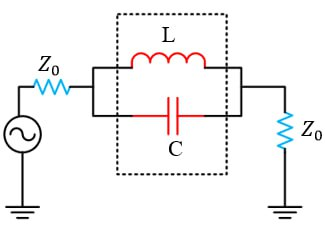
\includegraphics[scale=0.8]{Images/fig26.jpg}
 	\caption{معادل مداری ساختار زمین ناقص}
 	\label{fig26}
 \end{figure}
 
 در مقاله ی مد نظر ساختار انتخابی به صورت زیر میباشد: 
 
\begin{figure}
	\centering
	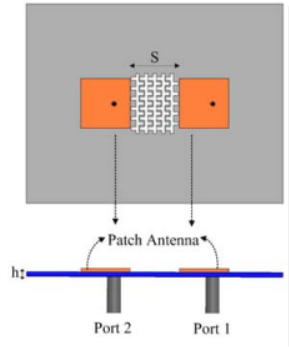
\includegraphics[scale=0.5]{Images/fig27.png}
	\caption{نمای بالایی و کناری از دو پچ آنتن به همراه DGS در صفحه ی زمین در آرایش E-Plain}
	\label{fig27}
 \end{figure}

\begin{figure}
	\centering
	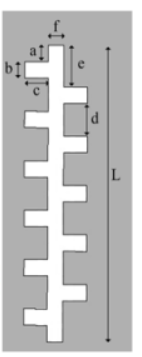
\includegraphics[scale=0.5]{Images/fig28.png}
	\caption{ارامتر های یک سلول DGS} % subcaption
	\label{fig28}
 \end{figure}
 
 
 با توجه به اینکه طراحی ارائه شده در مقاله مرجع
 \cite{carver1981microstrip}
 برای فرکانس کاری ۵ گیگاهرتز بهینه‌سازی شده است، جهت استفاده از این ساختار در فرکانس کاری مورد نظر این پروژه (۱.۴ گیگاهرتز)، لازم است ابعاد هندسی ساختار DGS به صورت متناسب اسکیل شوند. از آنجایی که ابعاد ساختارهای الکترومغناطیسی با طول موج رابطه مستقیم دارند، ضریب مقیاس ($\alpha$) از نسبت فرکانس‌ها محاسبه می‌شود: 
 
  \begin{align}
 	\label{eq:eq13}
 	\alpha = \frac{f_{\text{ref}}}{f_{\text{new}}} = \frac{5}{1.4} \approx 3.571
 \end{align}
 
 که در آن ۵ گیگ فرکانس کاری مقاله و 1.4 فرکانس جدید میباشد و در نتیجه ابعاد سلول DGS مقاله باید در 3.57 ضرب شوند.
 ابعاد قبل و بعد از محاسبه به صورت زیر میباشند : 
 \begin{center}
 \begin{tabular}{|c|c|c|}
 	\hline
 	74.55 & 21.0 & L \\
 	\hline
 	3.55 & 1.0 & a \\
 	\hline
 	3.55 & 1.0 & b \\
 	\hline
 	4.44 & 1.25 & c \\
 	\hline
 	8.17 & 2.3 & d \\
 	\hline
 	8.88 & 2.5 & e \\
 	\hline
 	3.55 & 1.0 & f \\
 	\hline
 \end{tabular}
 \end{center}
 
پس از اسکیل اولیه ابعاد بر اساس نسبت فرکانسی، شبیه‌سازی اولیه با پنج سلول DGS متوالی نتایج مطلوبی از نظر کاهش تزویج و تطبیق امپدانس در فرکانس هدف (۱.۴ گیگاهرتز) ارائه نداد. از این رو، بر اساس بررسی‌های تجربی، تغییرات زیر اعمال شد:
 
 
 
 